\documentclass[10pt,a4paper]{article}

\usepackage[margin=2.2cm,top=2.0cm,bottom=2.2cm]{geometry}
\usepackage[utf8]{inputenc}
\usepackage[T1]{fontenc}
\usepackage{lmodern}
\usepackage{titlesec}
\usepackage{booktabs}
\usepackage{array}
\usepackage{tabularx}
\usepackage{xltabular}
\usepackage{xcolor}
\usepackage{enumitem}
\usepackage{fancyhdr}
\usepackage{needspace}
\usepackage{tikz}
\usepackage[hidelinks]{hyperref}

% ---------- palette ----------
\definecolor{ink}{HTML}{22212B}
\definecolor{accent}{HTML}{3A2E6E}     % deep purple
\definecolor{amber}{HTML}{8A5D00}      % amber gold, text-safe 5.8:1
\definecolor{amberfill}{HTML}{C89211}
\definecolor{rule}{HTML}{D8D4E4}
\definecolor{muted}{HTML}{6B6878}
\definecolor{sevone}{HTML}{2A2050}\definecolor{sevtwo}{HTML}{5B46C4}
\definecolor{sevthree}{HTML}{9184E0}\definecolor{sevfour}{HTML}{CFC7F2}
\definecolor{info}{HTML}{6B6878}

% ---------- fonts: Latin Modern (lmodern), as in the research-paper build ----------
\newcommand{\display}{\sffamily}
\newcommand{\tabfont}{\relax}
\color{ink}

\titleformat{\section}{\display\normalsize\bfseries\color{accent}}{}{0pt}{}[\vspace{-0.55em}{\color{rule}\rule{\textwidth}{0.4pt}}]
\titlespacing*{\section}{0pt}{1.15em}{0.55em}
\setlist[itemize]{leftmargin=1.1em,itemsep=0.12em,topsep=0.25em}
\setlist[enumerate]{leftmargin=1.4em,itemsep=0.22em,topsep=0.25em}
\renewcommand{\arraystretch}{1.18}
\setlength{\parindent}{0pt}\setlength{\parskip}{0.3em}
\setlength{\tabcolsep}{6pt}
% Long \code{} tokens cannot hyphenate; let TeX stretch a little rather than overflow.
\setlength{\emergencystretch}{3em}

\pagestyle{fancy}\fancyhf{}
\lhead{\footnotesize\display\color{muted}WeConnect 2.0 — Quality Assurance}
\rhead{\footnotesize\display\color{muted}\thepage}
\renewcommand{\headrulewidth}{0pt}
\renewcommand{\headrule}{\vspace{-0.4em}{\color{rule}\rule{\headwidth}{0.4pt}}}

\newcommand{\code}[1]{{\ttfamily #1}}
\newcolumntype{L}{>{\raggedright\arraybackslash}X}
\newcolumntype{P}[1]{>{\raggedright\arraybackslash}p{#1}}
\newcommand{\grp}[1]{\multicolumn{2}{@{}l}{\display\small\bfseries\color{amber}#1}\\[0.15em]}

\begin{document}
\thispagestyle{empty}

% ================= header =================
{\display\fontsize{23}{26}\selectfont\color{accent}WeConnect 2.0 — Quality Assurance}\\[0.18cm]
{\color{accent}\rule{\textwidth}{1pt}}\\[0.16cm]
{\display\footnotesize\color{muted}Phases 1 and 2 \quad$\bullet$\quad 25 September 2026 \quad$\bullet$\quad For client review}

\vspace{0.45cm}

\begin{minipage}[t]{0.49\textwidth}
{\display\small\bfseries\color{accent}Status}\\[0.25em]
\begin{tabular}{@{}ll@{}}
Phase 1 — read-only & Complete \\
Phase 2 — transactional & Complete \\
Environment & Isolated, version-matched \\
Client data written & None \\
\end{tabular}
\end{minipage}\hfill
\begin{minipage}[t]{0.47\textwidth}
{\display\small\bfseries\color{accent}Coverage}\\[0.25em]
\begin{tabular}{@{}l>{\tabfont}r@{}}
Static routes swept & 235 / 235 \\
Dynamic routes & 17 / 17 \\
API endpoints probed & 71 \\
Self-verification controls & 46 \\
Business objects driven & 12 \\
\end{tabular}
\end{minipage}

\vspace{0.5cm}

\vspace{0.45cm}

{\color{rule}\rule{\textwidth}{0.5pt}}\\[0.30cm]
{\display\small\bfseries\color{accent}In brief}\\[0.35em]
{\footnotesize\raggedright
\textbf{What we found.} 119 findings. Three are confirmed breaches of the centre permission
boundary — an account acting on another centre's records, checked against the database. They share
one cause: the application code goes around a permission mechanism that works.

\vspace{0.25em}
\textbf{Fix these four first.} They are minutes of work each.
\code{WC-088} a one-word typo that breaks Enquiry Form status changes at two sites \textbullet{}
\code{WC-068} remove \code{allow\_guest} from three endpoints publishing your full API specification \textbullet{}
\code{WC-023} stop returning stack traces to callers \textbullet{}
\code{WC-121} replace the CORS wildcard with your two frontend origins.

\vspace{0.25em}
\textbf{What we need from you.} Sign the characterisation document — Part 1 is one page, and asks
you to confirm seven answers we worked out ourselves and answer \textbf{two} questions we could not.
Everything else waits on that.\par}

\vspace{0.15cm}
{\color{rule}\rule{\textwidth}{0.5pt}}

% ================= chart 1 =================
\section{Findings — 119 total}

\vspace{0.1cm}
\begin{center}
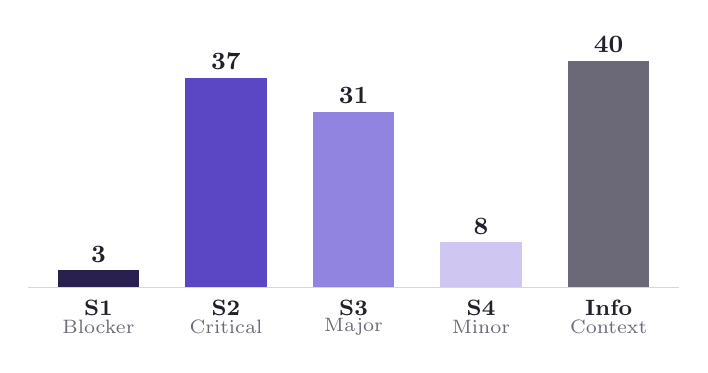
\begin{tikzpicture}[x=1.62cm,every node/.style={font=\footnotesize}]
\def\s{0.072}
\foreach \i/\v/\lab/\cap/\col in {%
  0/3/S1/Blocker/sevone, 1/37/S2/Critical/sevtwo, 2/31/S3/Major/sevthree,
  3/8/S4/Minor/sevfour, 4/40/Info/Context/info}{
  \fill[\col] (\i-0.32,0) rectangle (\i+0.32,{\v*\s});
  \node[font=\bfseries\small,color=ink] at (\i,{\v*\s+0.20}) {\v};
  \node[font=\bfseries\footnotesize,color=ink] at (\i,-0.26) {\lab};
  \node[font=\scriptsize,color=muted] at (\i,-0.50) {\cap};
}
\draw[rule] (-0.55,0) -- (4.55,0);
\end{tikzpicture}
\end{center}
\vspace{0.15cm}

{\footnotesize\color{muted}\raggedright
\mbox{\textbf{S1} Blocker — unauthorised action or data loss.}\quad
\mbox{\textbf{S2} Critical — security control missing or key logic failing.}\quad
\mbox{\textbf{S3} Major — significant defect with a workaround.}\quad
\mbox{\textbf{S4} Minor — presentation or hygiene.}\quad
\mbox{\textbf{Info} characterisation, no action.}\par}

% ================= S1 =================
\section{Critical (S1) — three confirmed breaches of the centre permission boundary}

We performed each of these on an isolated copy of the platform, signed in as an ordinary staff
account, against a record belonging to a centre that the account has no permission for. In each
case we then checked the database directly to confirm that the change had actually been made,
rather than relying on what the API reported. None of this was done against your data.

\vspace{0.5em}

% ---- S1-1 ----
{\display\small\bfseries\color{sevone}S1-1~{\footnotesize\color{muted}WC-095}\quad An account raised another centre's invoice into the financial approval pipeline}\\[0.35em]
The \code{sp} account is permitted for \textbf{QA East} and \textbf{QA West} only. It called
\code{raise\_invoice} on an invoice owned by \textbf{QA North}. The platform accepted the call and
advanced the invoice through its approval workflow.

\vspace{0.3em}
{\footnotesize
\begin{tabularx}{\textwidth}{@{}p{2.45cm}L@{}}
\textbf{Endpoint} & \code{youth\_skilling.api.invoice.raise\_invoice} — \code{PUT} \\
\textbf{Replied} & \code{success\_key:1} — "Skilling Invoice SK-INVOICE-00003 raised successfully." \\
\textbf{Database after} & \code{current\_status = Raised}, \code{approval\_status = Verification Pending} \\
\textbf{Reproduce} & \code{reproductions/s1-invoice-raise.mjs} \\
\end{tabularx}\par}

\vspace{0.35em}
\textbf{Why it matters.} The invoice has entered the financial approval queue, and the account
that put it there has no authority over the centre that owns it. The endpoint takes the centre from
the request and checks only that the invoice exists under that centre. It does not check whether
the caller is permitted for that centre.

\textbf{Fix.} Take the centre from the caller's own permissions rather than from the request,
and remove the \code{ignore\_permissions} flag from the save so that the framework's own check
applies.

\vspace{0.8em}
% ---- S1-2 ----
{\display\small\bfseries\color{sevone}S1-2~{\footnotesize\color{muted}WC-084}\quad An account closed another centre's batch}\\[0.35em]
The same account, with the same permissions, called \code{close\_batch} on a batch owned by
\textbf{QA North} and closed it.

\vspace{0.3em}
{\footnotesize
\begin{tabularx}{\textwidth}{@{}p{2.45cm}L@{}}
\textbf{Endpoint} & \code{youth\_skilling.api.batch\_management.close\_batch} — \code{POST} \\
\textbf{Replied} & \code{success\_key:1} — "Batch closed successfully." \\
\textbf{Database after} & \code{batch\_status = Closed} \\
\textbf{Reproduce} & \code{reproductions/s1-batch-close.mjs} \\
\end{tabularx}\par}

\vspace{0.35em}
\textbf{Why it matters.} Closing a batch completes it, which affects the status of the young
people enrolled in it and the invoicing that follows. The endpoint already reads the batch's owning
centre in order to build its reply, but it does not compare that centre against the centres the
caller is permitted for.

\textbf{Fix.} Compare the batch's centre against the caller's permitted centres before closing
it, and remove the \code{ignore\_permissions} flag from the save.

\vspace{0.8em}
% ---- S1-3 ----
{\display\small\bfseries\color{sevone}S1-3~{\footnotesize\color{muted}WC-048}\quad An account read another centre's youth counselling records}\\[0.35em]
An Outreach Coordinator account, permitted for two centres, requested the counselling list and
received \textbf{ten of ten records from centres it has no permission for}. Each record named a
youth and included the type and outcome of their counselling session, along with free-text
remarks about them.

\vspace{0.3em}
{\footnotesize
\begin{tabularx}{\textwidth}{@{}p{2.45cm}L@{}}
\textbf{Endpoint} & \code{facilitator\_and\_counsellor.api.counselling.list.get\_counselling\_list} \\
\textbf{Replied} & HTTP 200 — 10 of 10 records outside the caller's permitted centres \\
\textbf{Confirmed} & Reproduced three times; cause verified against the live platform, read-only \\
\textbf{Fields returned} & \code{youth\_name}, \code{counselling\_type}, \code{remarks}, \code{last\_call\_remarks}, \code{status}, and eight more \\
\end{tabularx}\par}

\vspace{0.35em}
\textbf{Why it matters.} These records concern youth and include counselling notes about
them. They were released across a permission boundary that the platform itself publishes to the
account at sign-in. We would treat this as a data-protection issue as well as a software defect,
and it may carry reporting obligations that are for the foundation to assess.

\textbf{The cause here is different from the other two, and so is the remedy.} The handler
already reads the caller's permitted centres and filters correctly on them. That filter is never
reached, because of the line immediately above it, which returns early for any caller holding the
\code{System Manager} role. Staff accounts hold that role because the permission model gives them
no working alternative: of the 293 doctypes the platform installs, 178 grant permissions to
\code{System Manager} and no other role, and the remaining 115 grant none at all.

\textbf{Fix.} Remove the role check from this and similar handlers. That change has to be made
together with proper per-role permissions on the doctypes, because on its own it would leave staff
accounts unable to see anything at all. The next section sets out the wider position.

\vspace{0.4em}
{\footnotesize\color{muted}We recorded only the names of the fields returned and the number of
records. No values from any youth's record were copied into this report or into any file we
hold.\par}

\vspace{0.5em}
All three share the same underlying cause. Two of them are write operations that switch the
permission check off, and the third is a read operation that skips it for a role that every account
holds. Changing how authorisation is enforced would address all three together, rather than
requiring three separate fixes.

% ================= systemic =================
\Needspace{14\baselineskip}\section{The underlying cause}

\begin{minipage}[t]{0.55\textwidth}
\vspace{0pt}
\raggedright
The framework's own permission mechanism is working correctly. When a write goes through the
ordinary save path, an attempt to change another centre's record is refused, and the error names
the centre that blocked it. This holds even for accounts that carry the \code{System Manager} role.
In every case we found, the problem is that the application code goes around that mechanism rather
than through it. It does so in two ways, and a third gap sits underneath both.

\vspace{0.4em}
{\display\small\bfseries\color{accent}On writes}\\[0.15em]
Thirty endpoints that change data pass the \code{ignore\_permissions} flag to the call that writes,
which switches the framework's check off, and they perform no check of their own beforehand.
\begin{itemize}
  \item We called 36 of them as an ordinary user. None refused the call.
  \item Driving the state-changing ones against another centre's records, three made the change and
        none refused; two could not be judged because the test data did not support them. Counting
        the two critical findings above, five endpoints are confirmed to change another centre's
        data.
  \item Fifteen of the 36 also return a server error, with a stack trace, when called with no
        input at all.
\end{itemize}

{\display\small\bfseries\color{accent}On reads}\\[0.15em]
Filtering by centre is skipped for any caller holding the \code{System Manager} role. We counted 45
places where this happens, across 26 files in seven of the eight applications. The filters
themselves are present and correct; they simply sit inside a condition that excludes that role.
This is what caused the counselling finding above.

{\display\small\bfseries\color{accent}On the records themselves}\\[0.15em]
The doctypes define no rules of their own, so nothing catches what the endpoints let through. Every
one of 174 attempted status changes was accepted across six doctypes, including \code{Paid} moving
back to \code{Not Raised Yet} on an invoice. Ten of twelve self-contradictory values were stored
without complaint, among them a negative age, a birth date in the future and a negative course cost.
Constraints written here would apply to every write path at once.
\end{minipage}\hfill
\begin{minipage}[t]{0.41\textwidth}
\vspace{0pt}
{\display\footnotesize\bfseries\color{accent}S2 findings by area}\\[0.35em]
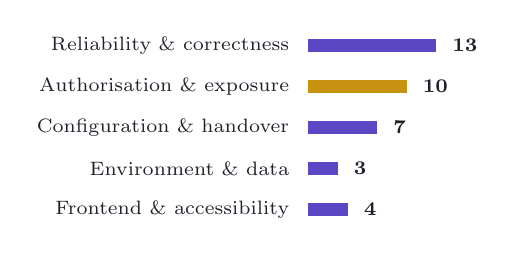
\begin{tikzpicture}[y=-0.52cm,every node/.style={font=\scriptsize}]
\def\w{0.125}
\foreach \i/\v/\lab/\col in {%
  0/13/Reliability \& correctness/sevtwo,
  1/10/Authorisation \& exposure/amberfill,
  2/7/Configuration \& handover/sevtwo,
  3/3/Environment \& data/sevtwo,
  4/4/Frontend \& accessibility/sevtwo}{
  \node[anchor=east,color=ink] at (0,\i) {\lab};
  \fill[\col] (0.12,\i-0.16) rectangle ({0.12+\v*\w},\i+0.16);
  \node[anchor=west,font=\scriptsize\bfseries,color=ink] at ({0.20+\v*\w},\i) {\v};
}
\end{tikzpicture}\\[0.6em]
{\scriptsize\color{muted}The highlighted group is the one we would address first.\par}
\vspace{0.5em}
{\display\footnotesize\bfseries\color{accent}Why this affects every account}\\[0.25em]
{\scriptsize Of the \textbf{293} doctypes the platform installs, \textbf{178} grant permissions to
\code{System Manager} and to no other role, and the remaining \textbf{115} grant none at all. A
staff account therefore cannot do its job without holding the role that turns the filtering off.\par}
\end{minipage}

\vspace{0.35em}
\textbf{What we would recommend, and in what order.} Authorisation should be enforced in one
place, through a decorator or a shared handler that every data-changing endpoint passes through,
rather than being written again in each endpoint. The role check should then be removed from the
read paths. Both of those changes depend on first giving each role real permissions on the
doctypes, because until that exists, removing the role check would leave staff unable to use the
platform at all. The validation and transition rules are independent of that sequence and can be
added at any point; they are also the cheapest of the three, because they are written once per
doctype rather than once per endpoint.

% ================= S2 table =================
\Needspace{8\baselineskip}\section{Critical findings (S2) — all 37, with remediation}

{\footnotesize
\begin{xltabular}{\textwidth}{@{}P{7.1cm}L@{}}
\toprule
\textbf{Finding} & \textbf{Fix} \\
\midrule
\endfirsthead
\toprule
\textbf{Finding} & \textbf{Fix} \\
\midrule
\endhead
\grp{Authorisation and data exposure — 10}
Mutating endpoints bypass permissions with no authorisation check (30 endpoints)
& Central authorisation: one decorator or base handler every mutating endpoint passes through. \\
Data scoping is disabled for \code{System Manager} at 45 sites in 7 of 8 apps — and 178 of 293 doctypes grant that role alone, so every staff account holds it
& Remove the role check from scoping paths, \emph{together with} a real per-persona permission model. Removing it alone locks staff out. \\
Any authenticated account, including an external partner, can trigger a bulk export of programme data to a Google Sheet
& Require an explicit administrative role for \code{sync\_to\_lcf\_mastersheet}, and log every invocation with the calling account. \\
Financial endpoints share the confirmed cross-centre write gap (\code{raise\_invoice}, \code{prepare\_tax\_invoice})
& Derive \code{center} from the caller's permitted scope, not from the request. \\
Personas receive records belonging entirely to centres they are not permitted for
& Two of the three handlers are the \code{System Manager} bypass above, not a missing filter. The third scoped correctly under test; its cause is unresolved. \\
Any authenticated user can delete any file by URL — no ownership check
& Verify the caller has permission for the file's parent document before deleting. \\
An unauthenticated endpoint attempts to provision a System Manager account
& Require an authenticated, authorised caller; never grant System Manager from it. Runtime blocks it today; the code path remains. \\
The complete API specification is published to unauthenticated callers
& Remove \code{allow\_guest=True} from the three \code{swagger\_spec} functions. \\
The permission design forces over-privileged accounts or bypasses permissions entirely
& Define per-persona roles with real doctype permissions, and stop relying on bypass. \\
\addlinespace[0.35em]
\code{add\_interest} writes every field the caller sends onto the Youth record, then saves with \code{ignore\_permissions=True}; confirmed setting a field the endpoint never declares
& Reject keys outside the declared set before writing — \code{update\_issue} in the same codebase already does this — and drop \code{ignore\_permissions}. \\
\grp{Reliability and correctness — 13}
Fields accept values that contradict themselves: negative ages, birth dates in the future, a capacity floor above its ceiling, negative course costs and instalment percentages of 150\% and $-$20\%
& Put the constraints on the doctype in a \code{validate} method, so every write path inherits them rather than each endpoint repeating them. \\
No state-transition control exists: 174 of 174 attempted status changes were accepted across six doctypes, including \code{Paid}$\rightarrow$\code{Not Raised Yet} and \code{Cancelled}$\rightarrow$\code{Paid} on invoices
& Define permitted transitions once on the doctype. Frappe's Workflow facility also supplies the transition history the invoice states need. \\
Enquiry Form status change is completely broken by a variable typo
& \code{ids = json.loads(ids)} — a one-word correction, plus a test that calls the endpoint. \\
Several endpoints return 403 over HTTP for every caller, Administrator included, though the function works when invoked directly
& Root-cause the API-layer rejection; these endpoints are unreachable over HTTP today. \\
Backend returns 500s under modest concurrency; sensitivity quantified by dose-response
& Size the worker pool for expected concurrency; return 503, not 500, under load. \\
SYC \code{/curriculum} data API returns 500
& Fix the server error in the curriculum data handler. \\
14 routes render blank on direct load; 2 group-based routes fail identically in both apps
& Root cause is null navigation state — read identifiers from URL parameters, not router state, and guard the read. \\
Opening the invoice screen attempts to create a tax invoice with no user action
& Load the screen with a GET; perform invoice preparation only on explicit user action. \\
Target Data API returns 404; widget shows ``Data not available''
& Restore the endpoint or remove the widget. \\
Endpoints crash rather than validate on missing input (15 of 36)
& Validate presence explicitly and return 400 naming the missing field. \\
A field returns the sentinel string \code{"NA"} where a list is expected
& Return \code{[]}. A field's type should not change with its emptiness. \\
State transitions are not guarded on current state
& Refuse to raise an already-raised invoice; guard each transition on the state it starts from. \\
No rate limiting on authenticated requests, on a backend that fails above three concurrent sessions
& Apply per-account and per-IP limits sized to the concurrency the backend can sustain, and paginate the unbounded youth endpoint. \\
\addlinespace[0.35em]
\grp{Configuration and handover — 7}
The permission model exists in no repository
& Export roles, role profiles and permission rules as app fixtures. \\
Runtime configuration required to operate the platform is not in the repositories
& Ship it as Frappe fixtures — the mechanism exists for exactly this. \\
Application code gates on roles that do not exist on a fresh install
& Ship the roles and the permission rules that reference them. \\
An installed application is absent from the repositories handed over
& Declare \code{required\_apps} in \code{hooks.py} and record the deployable set. \\
Attendance cannot be recorded on a fresh install — the code writes \code{Youth.status} values that ship in no master
& Ship the \code{Youth Status} master as fixtures, including every value the code writes. Until then every attendance save is rejected. \\
A ninth role profile (\code{Placement Youth Coordinator}) is routed to \code{/pyc/}, an application that does not exist
& Decide whether the persona is live. If it is, the application is missing; if not, remove it from the routing table and backend helpers. \\
Approval flows name at least 15 \code{Approval Category} records as string literals, and none ships — so every approval-driven flow fails on a fresh install
& Ship the categories as fixtures with the correct \code{ref\_doc}, replace the literals with constants, and reconcile \code{Move to Another Batch} / \code{Move to another Batch}. \\
\addlinespace[0.35em]
\grp{Environment and data protection — 3}
The environment\,$\rightarrow$\,API mapping is shifted by one in all 9 repositories: \code{.env.uat} calls dev, \code{.env.prod} calls uat, and no config names a production API
& Correct each environment's mapping and add the missing production configuration. Confirm which config each deployed frontend is built from. \\
Real programme data, including minors' records, is present in UAT
& Anonymise UAT, or confirm it is a production copy and restrict access accordingly. \\
A long-lived API secret is stored in \code{localStorage}
& Move to a short-lived, \code{httpOnly} session cookie. \\
\addlinespace[0.35em]
\grp{Frontend and accessibility — 4}
Server stack traces returned to callers in the standard error envelope
& Disable client-facing traceback rendering in the deployed site config. \\
The client-side auth guard is hardcoded to \code{true} — disabled in two persona apps
& Restore the guard and treat 403 like 401 in \code{axios-setup.js}. The backend does enforce auth, so this ships a broken shell, not an exposure. \\
Systematic WCAG critical violations, concentrated in shared navigation
& Correct the sidebar list markup, add \code{alt} to nav icons. One shared component fixes most instances. \\
The frontend is served with no security headers: no CSP, HSTS, \code{X-Frame-Options} or \code{X-Content-Type-Options}
& Add them at the nginx layer. CSP matters most here, because it is the control that limits what injected script can do with the token held in \code{localStorage}. \\
\bottomrule
\end{xltabular}\par}

% ================= what we need =================
% ================= where to start =================
\Needspace{10\baselineskip}\section{Where to start}

Every finding in the register carries an identifier and a priority. Priority is not severity: it
weighs how much the fix costs against what leaving it costs. Seventeen items are P1. Four of them
are a few minutes' work each and are worth doing this week, whatever else is decided.

\vspace{0.4em}
{\display\small\bfseries\color{accent}Quick wins — small changes, disproportionate effect}\\[0.35em]
\begin{tabularx}{\textwidth}{@{}l>{\raggedright\arraybackslash}X@{}}
\toprule
\textbf{ID} & \textbf{What to do} \\
\midrule
WC-088 & Correct \code{id = json.loads(id)} to \code{ids = json.loads(ids)}. It appears at two sites, not one; fixing either alone leaves the other path broken. Restores a feature that fails on every call. \\
WC-068 & Remove \code{allow\_guest=True} from the three specification endpoints. Takes the full API surface out of public view. \\
WC-023 & Turn off client-facing traceback rendering. Stops every error handing back internal paths and query structure. \\
WC-121 & Replace the CORS wildcard with an explicit list of your two frontend origins. One configuration line. \\
\bottomrule
\end{tabularx}

\vspace{0.5em}
{\display\small\bfseries\color{accent}The rest of P1}\\[0.35em]
{\footnotesize\raggedright
\textbf{Confirmed breaches:} WC-048, WC-084, WC-095 — the three in the section above.\quad
\textbf{Reachable without an account:} WC-077 provisioning, WC-078 file deletion by URL.\quad
\textbf{Data leaving its boundary:} WC-035 cross-centre records, WC-115 bulk export, WC-003 real PII in UAT.\quad
\textbf{Writes nobody asked for:} WC-038 invoice screen.\quad
\textbf{Unusable today:} WC-043 blank routes.\quad
\textbf{The programme of work:} WC-073, WC-079, WC-085, WC-105 — these are the authorisation rebuild, and the three confirmed breaches cannot close without them.\par}

\vspace{0.5em}
{\footnotesize\color{muted}\raggedright
The repository includes \code{verify/}, which re-checks the mechanically checkable findings against
your own environment and reports which are fixed. It needs only Node, issues read-only requests by
default, and is safe to point at any environment. A check that cannot run reports an error rather
than a pass.\par}

\Needspace{7\baselineskip}\section{What we need from you}

\begin{enumerate}[leftmargin=1.5em]
  \item \textbf{Fix the three critical findings and the two bypasses behind them.} The
        reproduction scripts included with this report will confirm when each one is closed.
  \item \textbf{Give each role proper permissions on the doctypes, then remove the
        \code{System Manager} check from the filtering code.} These two need to be done together.
        Because 178 of the 293 doctypes grant permissions to that role and no other, removing the
        check on its own would leave staff unable to use the platform.
  \item \textbf{Put the access-control configuration into the repositories.} Roles, role profiles,
        permission rules, naming series and the master data the code depends on should ship as
        fixtures. Four of the applications already use that mechanism for other settings, so this
        is a matter of extending what is there rather than introducing anything new.
  \item \textbf{Correct the environment configuration.} Each environment's frontend should point at
        its own API, and a production configuration needs to be added. We would also like to know
        which configuration each deployed frontend is currently built from, and whether the UAT
        database holds real programme data.
  \item \textbf{Review and sign the characterisation document.} It marks 15 decisions. We went back through them and answered what we could from the code and the data: seven are settled and need only your confirmation, six are narrowed to a smaller question, and \textbf{two genuinely need you} — whether there is an escrow or handover arrangement for \code{fintoo\_analytics\_bridge}, and whether each role has the right screens. Section 12 of that document sets out which is which, and what we found when we stopped asking and went looking.

  \item \textbf{Tell us how deletion is meant to work}, since no object can be deleted through the
        API at present, and whether \code{Placement Youth Coordinator} is a role you are still
        using.
\end{enumerate}

% ================= phase 3 =================
\Needspace{5\baselineskip}\section{Phase 3 — once the above is in hand}

The work below is what Phase 3 covers. It can begin once the characterisation document is
signed and the three critical findings are being addressed.


\begin{itemize}
  \item \textbf{Cross-browser and device matrix.} Playwright covers Chromium, Firefox and WebKit at
        no cost; BrowserStack is needed only for real iOS and Android hardware on a curated subset.
  \item \textbf{Continuous integration.} The suite on a defined trigger, with results visible to
        your team.
  \item \textbf{Regression closure.} Re-run the reproduction scripts against the remediated build
        and confirm each S1 closed.
  \item \textbf{Handover.} Documented suite, runbook and final closure report.
\end{itemize}

\end{document}
